\section{Introduction: architecture and services}

\subsection{Azure physical infrastructure}

\begin{itemize}
    \item {\bf DataCenter}
    \item {\bf Availability zone}: a physically separate datacenters within an Azure region. Each availability zone is made up of one or more datacenters equipped with independent power, cooling, and networking. An availability zone is set up to be an isolation boundary.
    \item {\bf region}: a geographical area that contains at least one datacenter that are nearby and networked together with a low-latency network
\end{itemize}

\subsection{Azure management infrastructure}

\begin{itemize}
    \item {\bf Ressource}: basic building block of Azure. Anything you create, provision, deploy, etc. is a resource. Virtual Machines (VMs), virtual networks, databases, cognitive services, etc. are all considered resources within Azure.
    \item {\bf Resource groups}: When a resource is crated, you’re required to place it into a resource group. a resource can only be in one resource group at a time. Some resources may be moved between resource groups. Resource groups can't be nested.  When and action (delete, grant or deny access\ldots) is applied  a resource group, that action will apply to all the resources within the resource group.
    \item {\bf subscription}: unit of management billing and scale. subscriptions allow  to logically organize  resource groups and facilitate billing. Azure subscription links to an Azure account, which is an identity in Microsoft Entra ID or in a directory that Microsoft Entra ID trusts.  subscriptions can be used to define boundaries around Azure products, services, and resources:
    \begin{itemize}
        \item Billing boundary:
        \item {\bf Access control boundary}: Azure applies access-management policies at the subscription level, and you can create separate subscriptions to reflect different organizational structures
    \end{itemize} 
    \item {\bf Management group}: container that help you manage access, policy, and compliance across multiple subscriptions. They are organized in a hierarchy.
\end{itemize}

\subsection{Compute services}

\begin{itemize}
    \item {\bf virtual machine}: provide infrastructure as a service in the form of a virtualized server and can be used in many ways.
    \item {\bf virtual desktop}:  is a desktop and application virtualization service. It provides centralized security management for users' desktops with Microsoft Entra ID. MFA can be enabled to secure sign-in. RBAC can be assigned to users to secure data.
    \item {\bf containers}:
        \begin{itemize}
            \item {\bf Container Instances}:
            \item {\bf Container Apps}:
            \item {\bf Kubernetes Service}:
        \end{itemize} 
    \item {\bf function}: is an event-driven, serverless compute option that doesn’t require maintaining virtual machines or containers.
    \item {\bf App Service}: is an HTTP-based service for hosting web applications, REST APIs, and mobile back ends.
        \begin{itemize}
            \item Web apps: 
            \item API apps
            \item WebJobs program or script that can be scheduled or run by a trigger
            \item Mobile apps
        \end{itemize}
    \item 
\end{itemize}

\subsection{Networking services}

\subsubsection{Virtual networking}
Virtual networks and virtual subnets enable Azure resources to communicate with each other, with users on the internet, and with on-premises client computers. They can be seen an extension of on-premises network with resources that link other Azure resources.

It allows the creation of multiple isolated virtual networks. When a virtual network is set up, a private IP space is defined by using either public or private (not internet routable) IP address ranges. This space can be devided into subnets.

For name resolution, the name resolution service built into Azure can be use or the virtual network can be configured to use either an internal or an external DNS server.

Incoming connections from the internet can be enabledby assigning a public IP address to an Azure resource, or putting the resource behind a public load balancer


Communication with on-prem ressources: three mechanisms for you to achieve this connectivity
\begin{itemize}
    \item {\bf Point-to-site virtual private network}
    \item {\bf Site-to-site virtual private networks} link on-prem VPN device or gateway to the Azure VPN gateway in a virtual network.
    \item {\bf ExpressRoute}: provides a dedicated private connectivity to Azure that doesn't travel over the internet. Useful for environments needing greater bandwidth and even higher levels of security.
\end{itemize}

By default, Azure routes traffic between subnets on any connected virtual networks, on-premises networks, and the internet. This setting can be override with:
\begin{itemize}
    \item Route tables 
    \item Border Gateway Protocol works with Azure VPN gateways, Azure Route Server, or Azure ExpressRoute to propagate on-premises BGP routes to Azure virtual networks.
\end{itemize}

Virtual networks enables to filter traffic between subnets by using the following approaches:
\begin{itemize}
    \item {\bf Network security groups}: resources that can contain multiple inbound and outbound security rules.
    \item {\bf Network virtual appliances}: specialized VMs that can be compared to a hardened network appliance.
\end{itemize}

virtual networks can be linked together by using virtual network peering.  Network traffic between peered networks is private, and travels on the Microsoft backbone network, never entering the public internet.

\subsubsection{VPN}
\href{https://learn.microsoft.com/en-us/training/modules/describe-azure-compute-networking-services/10-virtual-private-networks}{Describe Azure virtual private networks}

\subsubsection{ExpressRoute}
ExpressRoute allow to extend on-prem networks into the Microsoft cloud over a private connection, with the help of a connectivity provider. This connection is called an ExpressRoute Circuit. With ExpressRoute, connections can be established to Microsoft cloud services, such as Microsoft Azure and Microsoft 365. This allows you to connect offices, datacenters, or other facilities to the Microsoft cloud. Each location would have its own ExpressRoute circuit.

Connectivity can be from an any-to-any (IP VPN) network, a point-to-point Ethernet network, or a virtual cross-connection through a connectivity provider at a colocation facility. ExpressRoute connections don't go over the public Internet.

ExpressRoute supports four models:
\begin{itemize}
    \item CloudExchange colocation:
    \item Point-to-point Ethernet connection
    \item Any-to-any connection
    \item Directly from ExpressRoute sites
\end{itemize}

ExpressRoute is a private connection from on-pre infrastructure to Azure infrastructure. Even if you have an ExpressRoute connection, DNS queries, certificate revocation list checking, and Azure Content Delivery Network requests are still sent over the public internet

\subsubsection{DNS}
DNS is a hosting service for DNS domains that provides name resolution by using Microsoft Azure infrastructure

DNS is based on Azure Resource Manager, which provides features such as:
\begin{itemize}
    \item Azure RBAC
    \item Activity logs
    \item Resource locking prevents accidentally deleting or modifying critical resources
\end{itemize}

\subsection{Storage services}

\subsection{Identity, access and security}

\subsubsection{Entra ID}
Entra ID is Microsoft's cloud-based identity and access management service. It provides services such as:
\begin{itemize}
	\item Authentication: It also includes providing functionality such as self-service password reset, multifactor authentication, a custom list of banned passwords, and smart lockout services.
	\item Single sign-on: 
	\item Application management: both on-prem and cloud. Features like Application Proxy, SaaS apps, the My Apps portal, and single sign-on provide a better user experience.
	\item Device management: it supports the registration of devices  which enables devices to be managed through tools like Microsoft Intune. It also allows for device-based Conditional Access policies to restrict access attempts to only those coming from known devices, regardless of the requesting user account.
\end{itemize}

Active Directory can be connected with Microsoft Entra ID, enabling a consistent identity experience between cloud and on-premises. See \href{https://learn.microsoft.com/en-us/entra/identity/hybrid/}{Hybrid identity} In order to allow Active Directory users to use the same credentials in the on-premises environment and in the cloud, passwords hashes must be synchronized. There are 3 ways to perform synchronization in Azure AD:
\begin{itemize}
	\item \href{https://learn.microsoft.com/en-us/entra/identity/hybrid/connect/whatis-phs}{Password Hash Synchronization (PHS)}: This method synchronizes the password hashes from your on-premises AD to Entra ID
	\item \href{https://learn.microsoft.com/en-us/entra/identity/hybrid/connect/how-to-connect-pta}{Pass-through Authentication (PTA)}: PTA allows users to authenticate directly against your on-premises AD without storing passwords in the cloud.
	\item \href{https://learn.microsoft.com/en-us/entra/identity/hybrid/connect/whatis-fed}{Federated Authentication}: This method uses an on-premises identity provider, such as Active Directory Federation Services (AD FS) or PingFederate, to authenticate users
\end{itemize}

PHS is the most common option used by companies

There are two ways to sync:
\begin{itemize}
	\item {\bf Entra Connect}: synchronizes user identities between on-premises Active Directory and Microsoft Entra ID. Microsoft Entra Connect synchronizes changes between both identity systems, so you can use features like SSO, multifactor authentication, and self-service password reset under both systems.
	\item {\bf Entra Cloud Connect}: This is a lightweight agent that provides a cloud-based synchronization solution
\end{itemize}


\subsubsection{Entra Domain Services}
\href{https://learn.microsoft.com/fr-fr/entra/identity/domain-services/overview}{Entra Domain Services} service that provides managed domain services such as domain join, group policy, lightweight directory access protocol (LDAP), and Kerberos/NTLM authentication

It allows to run legacy applications in the cloud that can't use modern authentication methods. 

Entra Domain Services integrates with an existing Microsoft Entra tenant. This integration lets users sign into services and applications connected to the managed domain using their existing credentials. You can also use existing groups and user accounts to secure access to resources. These features provide a smoother lift-and-shift of on-premises resources to Azure.

When you create a Microsoft Entra Domain Services managed domain, you define a unique namespace. This namespace is the domain name. Two Windows Server domain controllers are then deployed into your selected Azure region. This deployment of DCs is known as a replica set

A managed domain is configured to perform a one-way synchronization from Microsoft Entra ID to Microsoft Entra Domain Services. You can create resources directly in the managed domain, but they aren't synchronized back to Microsoft Entra ID. In a hybrid environment with an on-premises AD DS environment, Microsoft Entra Connect synchronizes identity information with Microsoft Entra ID, which is then synchronized to the managed domain.

Applications, services, and VMs in Azure that connect to the managed domain can then use common Microsoft Entra Domain Services features such as domain join, group policy, LDAP, and Kerberos/NTLM authentication.

\subsubsection{Authentication methods}

\begin{itemize}
    \item Entra multifactor authentication:
    \item passwordless authentication:
        \begin{itemize}
            \item Windows Hello for Business
            \item Microsoft Authenticator app
            \item FIDO2 security keys
        \end{itemize}
\end{itemize}


\subsubsection{External identities}
An external identity is a person, device, service, etc. that is outside the organization. The external user’s identity provider manages their identity, and you manage access to your apps with Microsoft Entra ID or Azure AD B2C to keep your resources protected.
The following capabilities make up External Identities:

 \begin{itemize}
	\item Business to business (B2B) collaboration - Collaborate with external users by letting them use their preferred identity to sign-in to your Microsoft applications or other enterprise applications (SaaS apps, custom-developed apps, etc.). B2B collaboration users are represented in your directory, typically as guest users.
	\item B2B direct connect - Establish a mutual, two-way trust with another Microsoft Entra organization for seamless collaboration. B2B direct connect currently supports Teams shared channels, enabling external users to access your resources from within their home instances of Teams. B2B direct connect users aren't represented in your directory, but they're visible from within the Teams shared channel and can be monitored in Teams admin center reports.
	\item Microsoft Azure Active Directory business to customer (B2C) - Publish modern SaaS apps or custom-developed apps (excluding Microsoft apps) to consumers and customers, while using Azure AD B2C for identity and access management.
\end{itemize}

Depending on how you want to interact with external organizations and the types of resources you need to share, you can use a combination of these capabilities.

With Microsoft Entra ID, you can easily enable collaboration across organizational boundaries by using the Microsoft Entra B2B feature. Guest users from other tenants can be invited by administrators or by other users. This capability also applies to social identities such as Microsoft accounts.

You also can easily ensure that guest users have appropriate access. You can ask the guests themselves or a decision maker to participate in an access review and recertify (or attest) to the guests' access. The reviewers can give their input on each user's need for continued access, based on suggestions from Microsoft Entra ID. When an access review is finished, you can then make changes and remove access for guests who no longer need it.


\subsubsection{Conditional Access}

Conditional Access is a tool that Microsoft Entra ID uses to allow (or deny) access to resources based on identity signals. These signals include who the user is, where the user is, and what device the user is requesting access from.

Conditional Access also provides a more granular multifactor authentication experience for users

During sign-in, Conditional Access collects signals from the user, makes decisions based on those signals, and then enforces that decision by allowing or denying the access request or challenging for a multifactor authentication response.


Conditional Access is useful when you need to:

\begin{itemize}
	\item Require multifactor authentication (MFA) to access an application depending on the requester’s role, location, or network. For example, you could require MFA for administrators but not regular users or for people connecting from outside your corporate network.
	\item Require access to services only through approved client applications. For example, you could limit which email applications are able to connect to your email service.
	\item Require users to access your application only from managed devices. A managed device is a device that meets your standards for security and compliance.
	\item Block access from untrusted sources, such as access from unknown or unexpected locations.
\end{itemize}


\subsubsection{RBAC}
Azure provides built-in roles that describe common access rules for cloud resources. You can also define your own roles. Each role has an associated set of access permissions that relate to that role. When you assign individuals or groups to one or more roles, they receive all the associated access permissions.

Role-based access control is applied to a scope, which is a resource or set of resources that this access applies to.

\href{https://learn.microsoft.com/en-us/training/wwl-azure/describe-azure-identity-access-security/media/role-based-access-scope-4b12a8f3.png}{image}


Scopes include:
\begin{itemize}
	\item A management group (a collection of multiple subscriptions).
	\item A single subscription.
	\item A resource group.
	\item A single resource.
\end{itemize}

Observers, users managing resources, admins, and automated processes illustrate the kinds of users or accounts that would typically be assigned each of the various roles.


Azure RBAC is hierarchical, in that when you grant access at a parent scope, those permissions are inherited by all child scopes.

Azure RBAC is enforced on any action that's initiated against an Azure resource that passes through Azure Resource Manager. Resource Manager is a management service that provides a way to organize and secure your cloud resources.

Azure RBAC is enforced on any action that's initiated against an Azure resource that passes through Azure Resource Manager. Resource Manager is a management service that provides a way to organize and secure your cloud resources.

Azure RBAC uses an allow model. When you're assigned a role, Azure RBAC allows you to perform actions within the scope of that role. If one role assignment grants you read permissions to a resource group and a different role assignment grants you write permissions to the same resource group, you have both read and write permissions on that resource group.



\subsubsection{Identity Protection}

\href{https://learn.microsoft.com/en-gb/entra/id-protection/overview-identity-protection}{Identity Protection}  feature offers a supplementary layer of protections. Relying on the data they acquired from their position in organizations with Azure AD, Microsoft is able to detect risky user behaviors. These users can, then, be treated differently by Conditional Access Policies.

For example, a user can be identified as risky if he uses a password present in a leaked database.


\subsubsection{Entra ID security defaults}

Security defaults are a set of configurations that help protect you from identity-based attacks like password spraying and phishing.

Security defaults are designed for free-tier Entra ID tenants or those without Conditional Access features. While Conditional Access policies are fully customizable, security defaults are not. 

Security defaults offer the following controls:
\begin{itemize}
    \item Require all users to register a multi-factor authentication method
    \item Require administrators to log in using multifactor authentication (MFA)
    \item Require all users to log in using MFA to access: 
        \begin{itemize}
            \item Azure portal
            \item Microsoft Entra admin center
            \item Azure PowerShell
            \item Azure CLI
        \end{itemize}
    \item Disable legacy protocol authentication meaning that clients using IMAP, SMTP or POP3 will be rejected
\end{itemize}

\subsubsection{Password protection for Active Directory}
Azure AD offers the possibility to define password policies, which can be enforced on the on-premises Active Directory. This is handled by servers called Azure AD Password Protection Proxy Service and agents deployed on domain controllers.

\begin{figure}[!ht]
    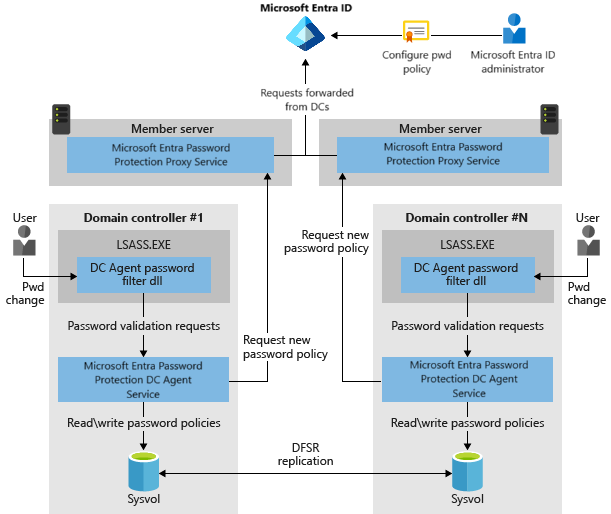
\includegraphics[width=\linewidth]{azure/knowledge/images/azure-ad-password-protection.png}
    \caption{Microsoft Entra Password Protection}
    \label{fig:azure-ad-password-protection}
\end{figure}

\subsubsection{Entra Privileged Identity Management}
\href{https://learn.microsoft.com/en-us/entra/id-governance/privileged-identity-management/pim-configure}{Entra Privileged Identity Management}

\subsubsection{Logging}
Azure Entra ID Portal has a Monitoring section where sign-in attempts and configuration changes are traced. It is possible to send those logs to Azure Logs Analytics, for further treatment, without subscribing to a premium license.


\subsection{Entra Connect}
Entra Connect has to be installed on a server from the Active Directory forest. Password hashes of Active Directory users do not transit over the network. A hash of each password hash is being sent instead.

Two accounts are automatically created by Azure AD Connect:
\begin{itemize}
    \item 
        \verb+MSOL_deeb213ff4bb+ in the Active Directory.
    \item
        \verb+Sync_SYNC01_deeb213ff4bb+ in Azure AD.
\end{itemize}

\verb+SYNC01+ being the hostname of the on-premises server where Azure AD Connect is installed and \verb+deeb213ff4bb+, an id, which changes for each environment.

In order to perfom the synchronization, the two accounts require high privileges over both environments. In the second part of this article, a way to compromise an Active Directory domain configured with PHS is shown.

\subsection{Entra Kerberos}




\subsection{links}
\begin{itemize}
    \item \href{https://www.synacktiv.com/publications/azure-ad-introduction-for-red-teamers}{Azure AD introduction for red teamers}
    \item \href{https://learn.microsoft.com/fr-fr/entra/identity/hybrid/connect/reference-connect-accounts-permissions}{Azure AD Connect : Comptes et autorisations}
    \item \href{https://servicetrust.microsoft.com/}{Azure Trust Portal}
    \item \href{https://msportals.io/?search=}{list of Microsoft portals}
\end{itemize}
